\chapter{Revisão Teórica}
\label{cap:teo}

\section{Introdução a Lógica Modal}
\label{sec:l_gica_modal}
Neste capítulo, introduziremos brevemente a base do pensamento modal. 

A lógica modal é determinada semanticamente pela avaliação de necessidade e
possibilidade de uma proposição, levando em consideração diferentes possíveis
contextos (ou \emph{mundos}). Na literatura, representações análogas à de
necessidade e possibilidade são utilizadas para a avaliação de estados
epistemológicos, como por exemplo, conhecimento e crença,
respectivamente~\cite{belief}. Basicamente, uma proposição é \textit{necessária}
se ocorre em todos os possíveis mundos e \textit{possível} se ocorre em algum
mundo~\cite{chellas:modal_logic}.  A ideia é que
diferentes ações ou objetos podem ser verdadeiros em mundos diferentes, mas
qualquer ideia que ocorra em todos os possíveis mundos é necessária, enquanto a
que ocorre em pelo menos um mundo, é possível.

Os operadores utilizados são os mesmos já conhecidos da lógica proposicional
($\wedge$, $\vee$, $\rightarrow$ etc) com a inclusão de dois novos:
$\nec{\agent}$ e $\pos{\agent}$. Uma sentença da forma $\nec{\agent} \varphi$
(\textit{necessariamente} $\varphi$) é verdadeira se, e somente se, $\varphi$ é
uma proposição verdadeira em todos os possíveis mundos, de acordo com o agente
$\agent$; já uma sentença da forma $\pos{\agent} \varphi$
(\textit{possivelmente} $\varphi$) é verdadeira no caso em que $\varphi$ é uma
proposição verdadeira em algum possível mundo, de acordo com o agente $\agent$.

Uma ilustração válida para a lógica modal, é pensar em uma coleção de possíveis
mundos, incluindo nosso próprio, o mundo real, onde sentenças da linguagem são
possivelmente verdadeiras ou falsas. O propósito principal da lógica modal é
modelar a ocorrência verdadeira destas sentenças.

A lógica modal pode ser expressa de diferentes formas e contar com diferentes
axiomas através da ideia de sistemas, isto será explorado com mais detalhes 
na seção~\ref{sec:sistemas}. 

%Um dos sistemas mais simples conhecidos é o $S5$, e
%este será utilizado para introdução, e, posteriormente, sua estrutura será
%expandido para uma forma mais geral.

%Um modelo no sistema $S5$ é, portanto, uma tupla:
%<$W$,~$P$>
%onde $W$ é um conjunto de possíveis mundos e $P$ uma abreviação para a sequência
%infinita 
%$P_0,\ P_1,\ P_2,\ldots$
%de subconjuntos de $W$.
%Note que $W$ pode conter mundos que não estão presentes em nenhum dos conjuntos
%$P_n$; de fato, qualquer um desses conjuntos pode ser vazio.

%Definimos o valor da sentença (verdadeiro ou falso) de acordo com sua forma e em
%termos de um possível mundo em um modelo.
%Usamos a notação:
%\begin{equation}
    %\label{modal:truth}
    %\models ^{\mathcal{M}}_{\alpha} A 
%\end{equation}
%onde $A$ é uma sentença e $\alpha$ é um possível mundo em um modelo
%$\mathcal{M}=<W,P>$.
%A lei~\ref{modal:truth} é um resumo para: $A\ é\ verdadeiro\ em\ \alpha\ no
%modelo\ \mathcal{M}$.

%As condições de verdade estão expressas na Tabela~\ref{table:truth}.

%\begin{center}
    %\begin{table}[h!]
%\label{table:truth3}
%\caption{Valores de cláusulas}

    %\begin{tabular}{ll}

        %\vspace{2mm}
        %(1) & $\models ^{\mathcal{M}}_{\alpha} \mathbb{P}_n$ se e somente se $\alpha \in
        %P_n$ com $n=0,1,2,\ldots$\\
        %\vspace{2mm}
        %(2)  & $\models ^{\mathcal{M}}_{\alpha} \top$\\
        %\vspace{2mm}
        %(3)  & $\neg\ \models ^{\mathcal{M}}_{\alpha}\bot $\\
        %\vspace{2mm}
        %(4)  & $\models ^{\mathcal{M}}_{\alpha} \neg A$ se e somente se $\neg \
        %\models ^{\mathcal{M}}_{\alpha} A$\\
        %\vspace{2mm}
        %(5)  & $\models ^{\mathcal{M}}_{\alpha} A \wedge B\ sse\ ambos
        %\models ^{\mathcal{M}}_{\alpha} A\ e \models ^{\mathcal{M}}_{\alpha} B$ \\
        %\vspace{2mm}
        %(6)  & $\models ^{\mathcal{M}}_{\alpha} A \vee B\ sse\ pelo\ menos\ um
        %\models ^{\mathcal{M}}_{\alpha} A\ ou \models ^{\mathcal{M}}_{\alpha} B$ \\
        %\vspace{2mm}
        %(7)  & $\models ^{\mathcal{M}}_{\alpha} A \rightarrow B\ sse\ se\
    %\models ^{\mathcal{M}}_{\alpha} A\ entao \models ^{\mathcal{M}}_{\alpha} B$ \\
        %\vspace{2mm}
        %(8)  & $\models ^{\mathcal{M}}_{\alpha} A \leftrightarrow B\ sse\ 
        %\models ^{\mathcal{M}}_{\alpha} A\ sse \models ^{\mathcal{M}}_{\alpha} B$ \\
        %\vspace{2mm}
        %(9)  & $\models ^{\mathcal{M}}_{\alpha} \Box A\ sse\ \forall \beta \in
        %\mathcal{M}, \models ^{\mathcal{M}}_{\beta} A$\\
        %\vspace{2mm}
        %(10)  & $\models ^{\mathcal{M}}_{\alpha} \Diamond A\ sse\ \exists \beta \in
        %\mathcal{M}, \models ^{\mathcal{M}}_{\beta} A$\\

    %\end{tabular}
%\end{table}
%\end{center}

%Alguns esclarecimentos sobre essas definições podem ser úteis:
%\begin{itemize}
    %\item A cláusula (1) reflete a premissa sobre os conjuntos $P_0, P_1, P_2,
        %\ldots$ em um modelo: uma sentença at\^omica $\mathbb{P}_n$ é verdadeira
        %em um possível mundo $\alpha$ somente no caso em que $\alpha$ é um
        %elemento do conjunto $P_n$.
    %\item De acordo com a cláusula (2), a constante verdadeira $\top$ é sempre
        %válida em $\alpha$.
    %\item Por (3), a constante falsa $\bot$ é sempre falsa em $\alpha$.
    %\item A cláusula (4) afirma que a negação $\neg A$ é verdadeira em $\alpha$
        %se, e somente se, sua negação $A$ é falsa em $\alpha$.
    %\item A afirmação da cláusula (5) diz que uma conjunção $A \wedge B$ é
        %verdadeira em $\alpha$ somente no caso em que ambas sentenças, $A$ e
        %$B$ o são.
    %\item Já de acordo com a cláusula (6), uma disjunção $A \vee B$ é verdadeira
        %em $\alpha$ quando pelo menos uma das sentençãos, $A$ ou $B$ o é.
    %\item A inteção com a cláusula (7) é compreender que uma implicação $A \rightarrow
        %B$ é verdadeira em $\alpha$ desde que nunca ocorra que a sentença antecedente,
        %$A$, seja verdadeira ao mesmo tempo em que a consequente, $B$, seja
        %falsa.
    %\item Similarmente, na cláusula (8) a intenção se repete de ambos os lados,
        %ou seja, a condição $A \leftrightarrow B$ é verdadeira quando ambas
        %sentenças, $A$ e $B$, são verdadeiras, ou ambas são falsas.
    %\item A cláusua (9) formula a interpretação leibniziana de necessidade:
        %$\Box A$
    %\item Finalmente, de acordo com a cláusula (10), $\Diamond A$
%\end{itemize}

%Observe que as constantes $\top$ e $\bot$ são, na realidade, operadores de
%aridade zero. Abstrações necessárias para algumas simplificações que veremos
%mais a frente.

%Na Figura~\ref{figure:mundos_simples} está ilustrado um exemplo de modelo para a
%lógica modal. No exemplo, o modelo $\mathcal{M}$ possui três mundos, $\alpha$,
%$\beta$ e $\omega$. Os conjuntos de mundos onde as sentenças at\^omicas são
%verdadeiras será expressado da seguinte forma:

%\begin{align}
    %P_0 &= \{\alpha, \beta, \omega\} \\
    %P_1 &= \{\alpha, \beta\}\\
    %P_2 &= \{\alpha, \omega\}\\
    %P_n &= \emptyset, \forall n > 2
%\end{align}

%Podemos, portanto expressar as seguintes sentenças para o modelo $\mathcal{M}$,
%sendo todas verdadeiras:

%\begin{align}
    %P_n &= \emptyset, \forall n > 2
%\end{align}

%Observe que não é verdade que $\Box \mathbb{P}_1$, pois $\mathbb{P}_1$ não é
%ocorre em $\omega$, ou seja, não satisfaz a condição de ocorrer em todos os
%possíveis mundos.

%\begin{figure}
%\begin{center}
%\label{figure:mundos_simples}
%\begin{tikzpicture}[scale=2]
    %\begin{pgfonlayer}{nodelayer}
        %\node [style=newstyle] (0) at (-3.75, 1) {$\mathbb{P}_0$};
        %\node[style=newstyle] (1) at (-2, 0.9) {};
        %\node[style=newstyle] (2) at (-0.25, 1) {};
        %\node[style=rect] (3) at (-2, 1) {};
    %\end{pgfonlayer}
%\end{tikzpicture}
%\caption{Exemplo lógica modal}
%\end{center}
%\end{figure}

%Uma sentença verdadeira em cada possível mundo em qualquer modelo é chamada
%\textit{sentença válida}. Usamos o símbolo $\models$ novamente, mas desta vez sem as
%marcações superior e inferior (para enfatizar que a sentença é verdadeira, sem
%importar o mundo ou o modelo), e escrevemos $\models A$ quando $A$ é uma
%sentença válida.
%Mais formalmente, então, definimos a validade de uma sentença da seguinte forma:

%\begin{equation}
    %\models A\ se,\ e\ somente\ se,\ para\ todo\ modelo\ \mathcal{M}\ e\ para\ 
    %qualquer\ mundo\ \alpha\ em\ \mathcal{M},\ temos\ que\ \models ^{\mathcal{M}}_\alpha 
%\end{equation}

%No estudo da lógica da necessidade e possibilidade, queremos saber quais são as
%sentenças válidas --- verdadeiras, sem se importar com interpretações, em
%qualquer mundo possível --- e quais não são. Por exemplo, podemos demonstrar que
%toda sentença da forma $\Box A \rightarrow A$ é válida, enquanto que nem toda
%sentença da forma $A \rightarrow \Box A$ o é.


%%% KEEP ON BABY

%%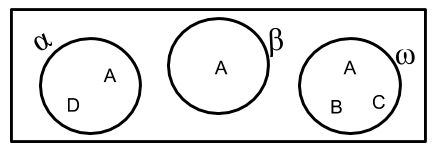
\includegraphics[scale=0.8]{imagens/ex_modal_simples.png}

%%\begin{tikzpicture}[node distance=2.5cm,auto,>=latex']
    %%\node [int, pin={[init]above:$v_0$}] (a) {$\frac{1}{s}$};
    %%\node (b) [left of=a,node distance=2cm, coordinate] {a};
    %%\node [int, pin={[init]above:$p_0$}] (c) [right of=a]
    %%{$\frac{1}{s}$};
    %%\node [coordinate] (end) [right of=c, node distance=2cm]{};
    %%\path[->] (b) edge node {$a$} (a);
    %%\path[->] (a) edge node {$v$} (c);
    %%\draw[->] (c) edge node {$p$} (end) ;
%%\end{tikzpicture}
%%\tikzset{simple/.style={thick}}



%??
\section{Preliminares lógicas}
\subsection{Sintaxe}
\label{sec:sintaxe}

Esta seção é dedicada a trazer o básico dos conceitos de sintaxe da linguagem da
lógica modal. As definições formais apresentadas podem ser úteis ao
entendimento.

\subsubsection{Sentenças} 
A linguagem proposicional clássica é formada por um conjunto enumerável de sentenças
\textit{at\^omicas} (ou símbolos proposicionais): 
\begin{equation}
\label{simb_prop}
    \mathcal{P} = \{\mathbb{P}_0, \mathbb{P}_1, \mathbb{P}_2, \ldots\}
\end{equation}
Estas são as sentenças mais simples possível.

Já as \textit{sentenças moleculares} (não-at\^omicas) são formadas por meio das
\textit{operações sintáticas}, ou \textit{operadores lógicos}: $\neg$, $\vee$ e
$\nec{\agent}$, para todo $\agent \in \Agents = \{1,\ldots, n\}$, $n \in \Nat$.
Observe que $\neg$ e $\nec{\agent}$ são operadores unários e $\vee$ é um operador
binário. Além disso, um conjunto de sinais de pontuação $\{(,)\}$ é usado para
evitar ambiguidade na leitura de sentenças.

Podemos então definir uma fórmula como uma combinação finita de sentenças
moleculares. A \textit{Linguagem Lógica Modal} é, portanto, equivalente ao seu
conjunto de \textit{fórmulas bem formadas}, definido a seguir.

\begin{definition} O conjunto de \textit{fórmulas bem formadas da linguagem modal}, denotado por
$FBF_{K}$ é definido indutivamente como segue:
    \label{def:fbf}

    \begin{enumerate}
    \item Os símbolos proposicionais estão em $FBF_{K}$;
    \item Se $\varphi \in FBF_{K}$, então $\neg \varphi$ e $\nec{\agent}\varphi$, $\agent \in \Agents$, estão em $FBF_{K}$; e
    \item Se $\varphi$ e $\psi$ estão em $FBF_{K}$, então $(\varphi \vee \psi)$ está em $FBF_{K}$.
    \end{enumerate}
    
\label{def:fbf}
\end{definition}

Outros operadores lógicos podem ser introduzidos como abreviações para fórmulas
construídas a partir dos operadores já definidos, como usual. Em particular,
neste trabalho as seguintes abreviações serão utilizadas: $(\varphi \land \psi)
= \neg (\neg \varphi \lor \neg \psi)$ (conjunção), $(\varphi \then \psi) = (\neg
\varphi \lor \psi)$ (implicação), $\pos{\agent} \varphi= \neg \nec{\agent} \neg
\varphi$ (possibilidade), $\cfalse = (\varphi \land \neg \varphi)$
(\emph{falsum}) e $\ctrue = \neg \cfalse$ (\emph{verum}). A precedência dos
operadores é dada na seguinte ordem (onde $\agent \in \Agents)$:
\begin{enumerate} 
    \item $\{\neg, \nec{\agent}, \pos{\agent}\}$ 
    \item $\{\wedge\}$ 
    \item $\{\vee\}$ 
    \item $\{\rightarrow\}$ 
\end{enumerate}

Quando não houver ambiguidade na leitura de uma fórmula, parênteses podem ser
omitidos.

Lógicas que envolvem vários agentes na lógica modal utilizam $n$ operadores, com
$n \in \mathbb{N}$, como descrito acima, são chamadas de \emph{lógicas
multimodais}. A lógica modal com um único agente, onde apenas temos os
operadores $\pos{1}$ e $\nec{1}$ (ou simplesmente $\pos{}$ e $\nec{}$), isto é,
onde $\Agents =\{1\}$, bem como a lógica proposicional clássica, onde $\Agents =
\{\}$, são, portanto, casos especiais da lógica multimodal.

O \emph{nível modal} de uma fórmula é o número máximo de ocorrências de
operadores modais sob o qual a fórmula ocorre. Por exemplo, em
$\nec{\agent}\pos{\agent}\mathbb{P}$, o nível modal de $\mathbb{P}$ é 2.

\subsubsection{Convenções} 
É importante definir algumas convenções para minimizar 
dúvidas que poderiam surgir em algumas expressões.
Expressões da forma $A_1 \wedge \ldots \wedge A_n$ e $A_1 \vee \ldots \vee A_n$
representam conjunções e disjunções arbitrárias mas não especificadas das
sentenças $A_1,\ldots,A_n$. O objetivo é deixar claro que tanto $\wedge$ como
$\vee$ obedecem as regras de associatividade lógica. 

\subsubsection{Fórmulas}
Agora que expressamos claramente a sintaxe que será utilizada na escrita de
sentenças e provas, podemos definir alguns conceitos que serão importantes mais
a frente.

A definição de \textit{fórmula} segue diretamente da sintaxe, e dizemos que é
qualquer sequência finita de símbolos lógicos. 

\begin{definition}[Fórmula bem-formada (FBF)]
    A lingagem lógica proposicional, denotada por $L_p$, é equivalente ao seu
    conjunto de fórmulas bem-formadas, denotado por $FBF_{L_P}$, que é definito
    recursivamente como segue:
    \begin{itemize}
        \item se $p \in P$, então $p \in FBF_{L_P}$
            \item se $\phi \in FBF_{L_P}$ e $\varphi \in FBF_{L_P}$, então: $\neg
                \phi,\ (\wedge), (\vee), (\rightarrow), (\leftrightarrow) \in FBF_{L_P}$, 
            
    \end{itemize}
\end{definition}

\begin{definition}[Forma Normal Negada (FNN)] Seja $\varphi \in FBF_{L_P}$, dizemos que $\varphi$ está na Forma Normal Negada (FNN) se contém apenas os conectivos $\neg$, $\wedge$ e $\vee$ e o
    conectivo de negação é aplicado apenas a símbolos proposicionais.
\end{definition}

A transformação em FNN é dada pelo seguinte procedimento:
\begin{enumerate}
    \item Substitua
    \item Substitua
    \item Aplique as leis de De Morgan
    \item Elimine
\end{enumerate}

%A simplificação de fórmulas aplica as seguintes regras de reescrita:
%\begin{itemize}
    %\item 
%\end{itemize}

\begin{definition}[Forma Normal Conjuntiva (FNC)]
    Seja $\varphi \in FBF_{L_P}$, dizemos que $\varphi$ está na Forma Normal
    Conjuntiva se é uma conjunção de cláusulas.
\end{definition}

A transformação de uma fórmula $\varphi$ em uma fórmula semanticamente
equivalente, $\varphi '$, na FNC, é dada pelo seguinte procedimento:

\begin{definition}[Forma Normal Disjuntiva (FND)]
    Seja $\varphi \in FBF_{L_P}$, dizemos que $\varphi$ está na Forma Normal
    Disjuntiva se é uma disjunção de conjunções de literais.
\end{definition}

A transformação de uma fórmula $\varphi$ em uma fórmula semanticamente
equivalente, $\varphi '$, na FND, é dada pelo seguinte procedimento:


\subsection{Semântica}
\label{semantics}

A ideia geral do significado de fórmulas na lógica proposicional modal pode ser
entendida, de forma simples, em termos de uma coleção de mundos possíveis, um conjunto
de atribuições de valores booleanos para cada símbolo proposicional em cada
mundo e relações de acessibilidade, que são definidas com base em um conjunto de
agentes.

Uma das estruturas mais estudadas em lógica modal corresponde à estrutura de
Kripke. 

\begin{definition}
    Uma \textbf{estrutura de Kripke}, para o conjunto de símbolos proposicionais
    $\mathcal{P}$ e o conjunto de agentes $\Agents = \{1,\ldots, n\}$, é
    uma tupla $\mathcal{M} = (W, \st_0, R_1,\ldots, R_n, \pi)$, onde:
   $W$ é um conjunto não-vazio de possíveis mundos; $\st_0 \in W$ é a raiz do modelo; 
   $\forall\agent \in \Agents, R_\agent \subseteq W \times W$ e
   $\pi : W \times \mathcal{P} \longrightarrow \{false, true\}$
    
\end{definition}

A partir da definição de estrutura de Kripke, podemos definir a satisfatibilidade
e a validade de uma fórmula.
\begin{definition}
    Seja $\mathcal{M} = (W, \st_0, R_1, \ldots, R_n, \pi)$ uma estrutura de Kripke sobre
    $\mathcal{P}$ e $\Agents$, e considere $w \in W$, $\mathbb{P} \in \mathcal{P}$
    e $\varphi$ e $\psi$ fórmulas bem formadas. A \textbf{relação de
    satisfatibilidade}, denotada por $\models ^{\mathcal{M}}_{w} \varphi$, entre
    o mundo $w$ e uma fórmula $\varphi$ no modelo $\mathcal{M}$, é definida
    indutivamente como se segue:
    \begin{itemize}
        \item $\models ^{\mathcal{M}}_{w} \mathbb{P}$ se e somente se, $\pi(w,\mathbb{P}) =
            true$;
        %\item $\models ^{\mathcal{M}}_{w} true$ e $\not\models ^{\mathcal{M}}_{w} false$; Você não precisa disso. Falso e verdateiro são abreviações.
        \item $\models ^{\mathcal{M}}_{w} \neg \varphi$ se e somente se,
            $\not\models ^{\mathcal{M}}_{w} \varphi$
            
        \item $\models ^{\mathcal{M}}_{w} \varphi \vee \psi$ se e somente se,
            $\models ^{\mathcal{M}}_{w} \varphi$ \texttt{ou} $\models
            ^{\mathcal{M}}_{w} \psi$
        \item $\models ^{\mathcal{M}}_{w} \nec{\agent} \varphi$ se e somente se,
            $\forall~t \in W$ com $\agent \in \Agents$  e $(w,t) \in R_\agent$,
            tem-se que $\models ^{\mathcal{M}}_{t} \varphi$. 
    \end{itemize}
\end{definition}

\begin{definition}
    Seja $\varphi \in FBF_{K}$, dizemos que $\varphi$ é
    \textbf{satisfatível} se existe um modelo $\mathcal{M}$ tal que $\models ^{\mathcal{M}}_{\st_0} \varphi$.  
\end{definition}

\begin{definition}
    Seja $\varphi \in FBF_{K}$, dizemos que $\varphi$ é
    \textbf{válida} se para todo modelo $\mathcal{M}$ temos que $\models ^{\mathcal{M}}_{\st_0} \varphi$.  
\end{definition}

Nós denotamos por $\depth(\st)$ o tamanho do caminho único entre $\st_0$ e  $\st$
através da união das relações de acessibilidade em $\model{M}$. 
Nós chamamos de \emph{camada modal} a classe de equivalência entre os mundos de
mesma profundidade em um modelo.

Observamos que verificar o problema de se verificar a satisfatibilidade de uma fórmula $\varphi$ em $\st_0$ pode ser reduzido ao problema de se checar a satisfatibilidade de todas as suas subfórmulas que ocorrem na camada modal de um modelo correspondente ao nível modal onde estas subfórmulas ocorrem (ver~\cite{Areces00tree-basedheuristics}). 

\section{Modelos padrões para a lógica modal}
\label{sec:modelos_padroes}

A ideia geral dada na seção~\ref{sec:l_gica_modal} é bastante simples, sendo
modelada basicamente em termos de uma coleção de possíveis mundos junto com uma
atribuição de valores booleanos, em cada mundo, a cada uma das sentenças
at\^omicas. Vimos que isso dá uma noção de validade um tanto restrita.
Nesta seção, iremos estender a definição leibniziana de necessidade e
possibilidade introduzindo o conceito de relações. O resultado é uma noção de
validade muito mais flexível.

Um modelo padrão será estruturado da seguinte forma:
\begin{equation}
    \label{eq:mod_padrao}
    \mathcal{M} =\ <W,R,P>
\end{equation}
onde $W$ representa o conjunto de possíveis mundos, $P$ representa a atribuição
dos subconjuntos de possíveis mundos a cada sentença at\^omica e o novo elemento
$R$, é uma relação entre possíveis mundos, ou seja, $R$ é uma relação binária em
$W$ ($R \subseteq W \times W$).

Escreveremos
\begin{equation}
    \alpha R \beta
\end{equation}
para dizer que o mundo $\beta$ está relacionado com, ou é relevante para, o
mundo $\alpha$. É importante ressaltar que $R$ pode ser qualquer tipo de relação
binária em $W$, nenhuma suposição é feita sobre sua estrutura.

As condições de verdade de sentenças não-modais, dadas na
Tabela~\ref{table:truth}, permanecem inalteradas. Já as relacionadas às
sentenças modais sofre uma pequena alteração, levando em conta agora, a relação
R da seguinte forma:

    \begin{table}[h!]
\label{table:truth2}
\begin{center}
    \caption{Condições de verdade: sentenças modais}
    \begin{tabular}{ll}
    Seja $\alpha$ e  \\

        \vspace{2mm}
        (1) & $\models ^{\mathcal{M}}_{\alpha} \mathbb{P}_n$ se e somente se $\alpha \in
        P_n$ com $n=0,1,2,\ldots$\\
        (2)  & $\models ^{\mathcal{M}}_{\alpha} $\\

    \end{tabular}
\end{center}
\end{table}

%\begin{figure}
%\begin{center}
%\label{figure:mundos_relacao}
%\begin{tikzpicture}[scale=2]
    %\begin{pgfonlayer}{nodelayer}
        %\node [style=newstyle] (0) at (-3.75, 1) {$\mathbb{P}_0$};
        %\node[style=newstyle] (1) at (-2, 1.4) {};
        %\node[style=newstyle] (2) at (-0.25, 1) {};
        %\node[style=newstyle] (4) at (-2, 0) {};
        %\node[style=rect2] (3) at (-2, 0.7) {M};
    %\end{pgfonlayer}
%\end{tikzpicture}
%\caption{Exemplo de modelo com relação}
%\end{center}
%\end{figure}


\subsection{Sistemas de lógica modal}
\label{sistemas}

%\subsubsection{Sistema $S5$}

%Nesta seção vamos examinar a necessidade e a possibilidade em $S5$ de um ponto
%de vista axiomático. Começamos com uma axiomatização baseada nos princípios das
%seções anteriores, ou seja, adotaremos como axiomas, ou teoremas básicos,
%quaisquer sentenças das seguintes formas:

%\begin{align}
    %T.& \\
    %5.& \\
    %K.& \\
    %Df\Diamond.& \\
    %PL.& 
%\end{align}

%E assumimos as seguintes regras de inferência:

%\begin{mathpar}
%\label{natrules1}
%(RN)~\inferrule{A}{\Box~A} 
%\end{mathpar}

%\begin{mathpar}
%\label{natrules1}
%(MP)~\inferrule{A \rightarrow~B, A}{B} 
%\end{mathpar}

%Por teorema, geralmente, queremos dizer qualquer sentença que possa ser provada
%com base nos axiomas e nas regras de inferência e denotamos como $\vdash A$ para
%dizer que a sentença $A$ é também um teorema.

%Podemos observar que $S5$, aqui formulado como um sistema dedutivo, inclui a
%lógica proposicional, ou seja, a seguinte regra de inferência pode ser derivada
%de dentro do sistema:

%\begin{mathpar}
%\label{natrules1}
%(RPL)~\inferrule{A_1, \ldots, A_n}{A}~(n \geq~0) 
%\end{mathpar}

%Para provarmos tal regra, mostramos que se a inferência de $A_1, \ldots, A_n$
%para $A$ é proposicionalmente correta, e cada um dos $A_1, \ldots, A_n$ é um
%teorema, então $A$ também é um teorema. A suposição de que a inferência é
%proposicionalmente correta implica que $A$ é verdadeiro em qualquer validação
%onde cada um dos $A_1, \ldots, A_n$ é verdadeiro, o que basicamente expressa que
%a sentença
%\begin{equation}
    %A_1 \rightarrow (\ldots(A_n \rightarrow A) \ldots)
%\end{equation}
%é uma tautologia (PL), ou seja, um teorema. Aplicamos a regra (MP) $n$ vezes, e
%concluímos que $A$ também é um teorema.

%Utilizamos o sistema $S5$ para ilustrar alguns conceitos iniciais de prova e
%regras de inferência. A seguir, iremos mostrar como aplicá-los a sistemas mais
%complexos da lógica modal.

%\subsubsection{Outros sistemas}
%\label{ssub:Outrossistemas}

%Os diferentes sistemas de lógica modal surgem em parte pela necessidade em diferentes
%tipos de aplicações e em parte porque nossas intuições sobre o que é necessariamente
%verdade ainda não estão completamente desenvolvidas. Originalmente, lógicas
%modais diferentes eram caracterizadas por conjuntos de axiomas distintos. 

%Definimos sistemas de lógica modal em termos do fecho sobre a regra de
%inferência (RPL), onde $A$ é uma consequência tautológica das sentenças $A_1,
%\ldots, A_n$.

%\begin{definition}[Sistema de lógica modal]
   %Um conjunto de sentenças é um \textit{sistema de lógica modal} se, e somente
   %se, é fechado sobre (RPL).
%\end{definition}

%Assim, um sistema de lógica modal é qualquer conjunto de sentenças fechado com
%respeito a todos os modos proposicionalmente corretos de inferência.
%Reservaremos a notação $\Sigma$ como uma variável para conjuntos de sequências
%que são sistemas de lógica modal, e, para simplicidade, constantemente iremos
%nos referir aos mesmos simplesmente como sistemas.

%Os teoremas em um sistema são simplesmente as sentenças que o mesmo contém.
%Escrevemos $\vdash_{\Sigma} A$ quando $A$ é um teorema de $\Sigma$.

%\begin{definition}[Teorema em sistemas modais]
    %$\vdash_{\Sigma} A$ se, e somente se $A \in \Sigma$.
%\end{definition}

%Como sistemas são simplesmente conjuntos de sentenças, a força de um sistema é medido em
%termos de inclusão: um sistema é pelo menos tão forte quanto um sistema $\Sigma$
%--- e denotaremos como um $\Sigma$-sistema --- somente no cso em que contém todo
%e qualquer teorema de $\Sigma$ (note que esta relação é reflexiva).

%\begin{theorem}
    %O conjunto de tautologias é definido a partir do axioma PL, definido na
    %seção anterior.\\
    %(1) PL é um sistema de lógica modal. \\
    %(2) Todo sistema de lógica modal é um PL-sistema. \\
    %(3) PL é o menor sistema de lógica modal.
%\end{theorem}
%Demonstração. $\qed$

%Podemos definir noções de \textit{dedutibilidade} e \textit{consistência}, em
%termos de teoremicidade. 

%Uma sentença $A$ é dedutível de um conjunto de
%sentenças $\Gamma$ e um sistema $\Sigma$ --- e escrevemos $\Gamma
%\vdash_{\Sigma} A$ --- se, e somente se, $\Sigma$ contém um teorema da forma:
%\begin{equation}
    %(A_1 \wedge \ldots \wedge A_n) \rightarrow A
%\end{equation}
%onde cada $A_i~(i=1,\ldots,n)$ dos antecedentes é uma sentença em $\Gamma$.

%Um conjunto de sentenças $\Gamma$ é consistente em $\Sigma$ --- e escrevemos
%$Con_{\Sigma}\Gamma$ --- somente no caso em que a sentença $\bot$ não é
%$\Sigma$-dedutível a partir de $\Gamma$.

%Mais formalmente:

%\begin{definition}[Dedutibilidade]
    
%\end{definition}

%\begin{definition}[Consistência]
    
%\end{definition}

%Teoremicidade, dedutibilidade e consistência, como definitos, possuem todas as
%propriedades esperadas, algunas das quais estão enumeradas no seguinte teorema.

%\begin{theorem} ~
    %\begin{enumerate}
        %\item $\vdash_{\Sigma}A\ sse\ \emptyset \vdash_{\Sigma}A$
        %\item $\vdash_{\Sigma}A\ sse\ \forall \Gamma, \Gamma \vdash_{\Sigma}A$
        %\item $Se\ \Gamma \vdash_{PL}A\ entao\ \Gamma \vdash_{\Sigma}A$
        %\item $Se\ A\in \Gamma\ entao\ \Gamma \vdash_{\Sigma}A$ \item $Se\ \Gamma
            %\vdash_{\Sigma}B\ e\ \{B\}\vdash_{\Sigma}A\ entao\ \Gamma
            %\vdash_{\Sigma}A$
        %\item $Se\ \Gamma \vdash_{\Sigma}A\ e \Gamma \in \Delta\ entao\ \Delta
            %\vdash_{\Sigma} A$
        %\item $\Gamma \vdash_{\Sigma}A\ sse\ existe\ um\ subconjunto\ finito\ 
            %\Delta\ de\ \Gamma\ tal\ que\ \Delta \vdash_{\Sigma}A$
        %\item $\Gamma \vdash_{\Sigma}A\rightarrow B\ sse \Gamma \vdash_{\Sigma}A$
        %\item $Con_{\Sigma}\ \Gamma\ sse\ existe\ um\ A\ tal\ que\ \neg \Gamma \vdash_{\Sigma}A$
        %\item $Con_{\Sigma}\ \Gamma\ sse\ nao\ existe\ A\ tal\ que\ ambos\ \Gamma
            %\vdash_{\Sigma}A \Gamma \vdash_{\Sigma}\neg A$
        %\item $Se\ Con_{\Sigma}\ \Gamma\ entao\ Con_{PL}\Gamma$
        %\item $Se\ Con_{\Sigma}\ e\ \Delta \in \Gamma\ entao\ Con_{\Delta}$
        %\item $Con_{\Sigma}\ \Gamma\ sse\ \forall \Delta \in \Gamma,
            %Con_{\Sigma}\Delta$
        %\item $\Gamma \vdash_{\Sigma}A\ sse\ Con\{\neg A\}$
        %\item $Con_{\Sigma}\Gamma \{A\}\ sse\ \neg \Gamma \vdash_{\Sigma}\neg A$
    %\end{enumerate}
%\end{theorem}

%Demonstração. $\qed$

%Iremos agora introduzir um conjunto dos sistemas mais conhecidos da lógica
%modal: $K$, $D$, $T$, $B$, $K4$, $S4$ além de retomarmos brevemente sobre o
%sistema $S5$ mencionado anteriormente. A definição destes sistemas utiliza a
%semântica de possíveis mundos.

%\begin{definition}[$L$-Válida]
    %Dizemos que o modelo $\mathcal{M} = <W, R, P>$ é baseado no quadro $<W,R>$.
    %Umafórmula $X$ é válida no modelo $\mathcal{M}$ se é verdadeira em todo
    %mundo de $W$. Uma fórmula $X$ é válida em um quadro se é válida em cada
    %modelo baseado naquele quadro. Finalmente, se $L$ é uma coleção de quadros,
    %$X$ é $L$-válida se $X$ é válida em cada quadro em $L$.
%\end{definition}

%Diferentes sistemas de lógica modal são caracterizados semanticamente como as
%fórmulas $L$-válidas, para $L$ classes em particular de quadros. Para
%exemplificar, o sistema chamado $T$ é caracterizado pela classe de quadros que
%contenham a propriedade de que todo mundo é acessível por ele mesmo. Este tipo
%de propriedade pode vir a ser útil posteriormente e está definida a seguir,
%junto com outras propriedades de valor similar.

%\begin{definition}
    %Seja $Q = <W,R>$ um quadro. Dizemos que $Q$ é:
    %\begin{enumerate}
        %\item \textit{reflexivo}
        %\item \textit{simétrico}
        %\item \textit{transitivo}
        %\item \textit{serial}
        %\item \textit{euclidiano}
    %\end{enumerate}
    
%\end{definition}

%O sistema $T$, mencionado acima, é caracterizado pela classe de quadros
%reflexivos. A Tabela~\ref{table:condicoes_quadro} informa as classes de quadros
%aos quais os demais sistemas são caracterizados.

%\begin{table}[h!]
    %\begin{center}
        %\label{table:condicoes_quadro}
        %\caption{Alguns sistemas padrões de lógica modal}
        %\begin{tabular}{ll}
            %\hline
            %Sistema & condições para classe de quadros \\
            %\hline
            %$K$  & sem condições \\  
            %$D$  & serial \\ 
            %$T$  & reflexivo \\ 
            %$B$  & reflexivo, simétrico\\ 
            %$K4$ & transitivo \\  
            %$S4$ & reflexivo, transitivo \\  
            %$S5$ & reflexivo, simétrico, transitivo \\
            %\hline
        %\end{tabular}
    %\end{center}
%\end{table}

%A figura~\ref{fig:subsistemas} mostra como os sistemas de lógica modal
%mencionados nesta seção estão
%relacionados entre si, ou seja, se existe uma seta partindo de $L$ e chegando em $J$, sendo $L$ e
%$J$ sistemas, podemos dizer que $J$ é um $L$-sistema.

%%\begin{figure}
%%\label{fig:subsistemas}
%%\begin{center}
%%\begin{tikzpicture}
    %%\begin{pgfonlayer}{nodelayer}
        %%\node  (0) at (0, 2) {S5};
        %%\node  (1) at (-2, 0.7) {B};
        %%\node  (2) at (2, 0.7) {S4};
        %%\node  (3) at (-2, -0.6) {T};
        %%\node  (4) at (-2, -1.8) {D};
        %%\node  (5) at (2, -1) {K4};
        %%\node  (6) at (0, -2.7) {K};
        %%\path[->,thick] (1) edge node {} (0)
        %%(2) edge node {} (0)
        %%(3) edge node {} (1)
        %%(5) edge node {} (2)
        %%(3) edge node {} (2)
        %%(4) edge node {} (3)
        %%(6) edge node {} (4)
        %%(6) edge node {} (5);

    %%\end{pgfonlayer}
%%\end{tikzpicture}
%%\end{center}
%%\caption{Subsistemas}
%%\end{figure}

%\subsection{Lógica Multimodal}
%\label{sub:lógica_multimodal}


%\subsubsection{Estrutura de Kripke}

%Uma das estruturas mais estudadas em lógica modal corresponde à estrutura de
%Kripke. Uma estrutura de Kripke para $P$ e $A_n = \{1, \ldots, n\}$ é dada da seguinte forma:
%\begin{equation}
%\mathbb{M} = <W,\ R_1, \ldots,\ R_n, \pi>
%\end{equation}
%onde:
%\begin{itemize}
    %\item $W$ é um conjunto não-vazio de possíveis mundos
    %\item para todo $a \in A_n, R_a \subseteq W \times W$
    %\item $\pi: W \times P \longrightarrow \{Falso, Verdadeiro\}$
%\end{itemize}

%%\begin{figure}
%%\label{fig:kripke}
    %%\begin{center}
        %%\begin{tikzpicture}
            %%\begin{pgfonlayer}{nodelayer}
                %%\node [style=bolinha] (0) at (0, 2) {};
                %%\node [style=bolinha] (1) at (-2, -1) {};
                %%\node [style=bolinha] (2) at (2, -1) {};
                %%\path[->] (0) edge node {} (0)
                %%(1) edge node {} (1)
                %%(2) edge node {} (2);
                %%\path[<->] (0) edge node {} (1)
                %%(0) edge node {} (2);
            %%\end{pgfonlayer}
        %%\end{tikzpicture}
    %%\end{center}
    %%\caption{Estrutura de Kripke}
%%\end{figure}


\section{Resolução}
\label{sec:resolucao}
Informalmente, uma prova é um argumento que convence. Formalmente, uma prova é
uma fórmula, é um objeto finito construído de acordo com regras de sintaxe
fixadas que fazem referência unicamente à estrutura das fómulas e não ao seu
significado pretendido. As regras sintáticas que definem as provas especificam o
que chamamos de \textit{procedimento de prova}.
Um procedimento de prova é \textit{sólido} para uma lógica em particular se
para qualquer fórmula que possuir uma prova, esta fórmula se trata de uma
fórmula válida nesta lógica. Um procedimento de prova é \textit{completo} para
uma lógica se toda fórmula válida daquela lógica possui uma prova. Dessa forma,
um procesimento sólido e completo de provas nos permite constuir
``testemunhas'', chamadas de provas, de que determinada fórmula é válida.

Existem inúmeros tipos de procedimentos de provas. Genericamente, podemos
dividi-los em duas categorias: \textit{sintéticos} e \textit{analíticos}. Os
termos são sugestivos, mas não extremamente precisos. Uma procedimento de prova
analítico decompõe uma fórmula em partes mais simples. Um procedimento de prova
sintético, por outro lado, constrói uma prova até a fórmula que se deseja obter a
demonstração.
O primeiro tende a ser mais facilmente aplicado, já que o espaço em que se
trabalha é limitado: nunca olha-se para muito longe do escopo onde se encontra a
fórmula que se está tentando prova. Já o segundo costuma ser mais utilizado por
produzir provas especialmente elegantes.

O exemplo mais comum de procedimento sintético é um \textit{sistema de axiomas}.
Algumas fórmulas são tomadas como axiomas, uma prova começa com esses axiomas e,
usando regras de inferência definidas, que produzem novas fórmulas, é construído
uma sequência de fórmulas que finalmente termina na fórmula que se está tentando
provar.

\textit{Sistemas Tableaux} são um dos mais comuns procedimentos de prova
analítica. Para provar uma fórmula, precisamos inicialmente negá-la, analisando
as consequências de ser tomada tal ação, utilizando uma estrutura em forma de
árvore. Este tipo de sistema é conhecido como \textit{sistemas de refutação}.
Se, as consequências resultarem em algo impossível, pode-se concluir que a
fórmula original está provada. Falaremos mais sobre este sistema na
Seção~\ref{sub:tableaux}.


\subsection{Resolução Clausal}
\label{clausal}

Este método de prova é conhecido como um procedimento refutacional: para
podermos provar a fórmula $\varphi$, nós transformamos a sua negação ($\neg
\varphi)$ na Forma Normal, para, então, aplicarmos as regras de inferência ao
conjunto de cláusulas resultante com a finalidade de gerar a cláusula vazia, que
indicará uma contradição no conjunto de cláusulas, provando a fórmula original. 

Existe uma forma normal específica para a lógica modal $K$, a Forma Normal
Separada para Sistemas Normais baseada em Níveis Modais \snf{K}, que faz com
que os contextos referentes aos diferentes agentes sejam separados. As regras de
transformação e a prova de correção do método de tradução para $\snf{K}$ podem
ser encontrados em~\cite{DBLP:conf/tableaux/NalonHD15}. Uma fórmula em $\snf{K}$
é representada por um conjunto de cláusulas, que são verdadeiras em todos os
mundos alcançáveis.  Uma fórmula em $\snf{K}$ possui o seguinte formato:
\begin{equation} \bigwedge_i ml: C_i \end{equation} onde cada $C_i$ é uma
    cláusula e $ml$ é o nível modal onde a cláusula ocorre.

As seguintes definições também são necessárias:

\begin{definition} \textit{Literal} é um símbolo proposicional $\mathbb{P}$ ou
sua negação $\neg \mathbb{P}$. Denotamos por $\cal{L}$ o conjunto de todos os
literais.  \end{definition}

\begin{definition} Um \textit{literal modal} é uma fórmula na forma
$\nec{\agent} l$ ou sua negação $\neg \nec{\agent} l$, sendo $l$ um literal e
com $\agent \in \Agents$.  \end{definition}

Uma cláusula pode assumir um dos seguintes formatos:

\begin{itemize} \item Uma cláusula de literais:

        \begin{center} $ml: \bigvee^r_{b=1} l_b$ \end{center} \item Uma cláusula
                $\agent$-positiva:

        \begin{center} $ml: l' \Rightarrow \nec{\agent} l$ \end{center} \item
                Uma cláusula $\agent$-negativa:

        \begin{center} $ml: l' \Rightarrow \neg \nec{\agent} l$ \end{center}
    \end{itemize} onde $l$, $l'$ e $l_b \in \mathcal{L}$, $\agent \in \Agents$,
    $r \in \mathbb{N}$ e $ml \in \Nat$.

Uma vez que as fórmulas estejam em sua forma normal, o método de resolução pode
ser aplicado, ou seja, as regras de inferência podem ser aplicadas ao conjunto
de cláusulas resultante. Nós omitiremos a descrição do método, que pode ser
encontrada em \cite{DBLP:conf/tableaux/NalonHD15}, uma vez que para os objetivos
deste trabalho precisamos tão somente da definição da forma normal apresentada
acima.

\subsection{Tableaux}
\label{sub:tableaux}
Métodos de demonstração utilizando tableaux são frequentemente utilizados, com
sucesso, em lógica modal para prover procedimentos de decisão. O tableaux
consiste em uma prova representada graficamente na forma de árvore. É um método
analítico baseado na prova por contradição~\cite{fit:tableaux}.

\begin{definition}
    Uma \textbf{regra $\sigma$} no método tableaux consiste em um numerador $N$,
    acima da linha, e uma lista (finita) de denominadores $D_1, D_2,
    \ldots, D_k$ (abaixo da linha), separados por barras verticais. O numerador e
    cada denominador são um conjunto finito de fórmulas~\cite{tableaux:def}.
\end{definition}
 
Cada regra é lida de cima para baixo, e se o numerador é satisfatível,
então um dos denominadores também o é. O numerador de cada regra do
tableaux contém uma ou mais fórmulas distintas chamadas de \textit{fórmula(s)
principal(is)}. Um \textit{cálculo baseado em tableaux} para uma lógica $L$ ($\mathcal{C}_L$) 
é um conjunto finito de regras~\cite{clausal_tableaux}.

Dado um $\mathcal{C}_L$, um tableaux para uma fórmula $\varphi$ é uma árvore tal
que sua raiz contém $\varphi$ e os outros nós contém conjuntos finitos de
fórmulas obtidas a partir de seus nós-pais, através da ativação de uma regra de
$\mathcal{C}_L$. Um \textit{ramo}, em um tableaux, representa um caminho entre a
raiz da árvore e um de seus nós. %% você não precisa de regra de blocking para
K; o artigo que você leu, do Goré, é para combinações envolvendo 4.

\begin{definition}
Seja $\Delta$ um conjunto de regras de tableaux. Dizemos que $\psi$ é
\textbf{obtível a partir de} $\varphi$ por aplicações de regras em $\Delta$ se existe
um tableaux para $\varphi$, que utiliza somente as regras contidas em $\Delta$, e possui
um nó que contém $\psi$. 
\end{definition}

\begin{definition}
    Um ramo em um tableaux é dito \textbf{fechado} se seu nó final
    contém apenas $\bot$. Um tableaux é dito \textbf{fechado} se cada um de seus
    \textit{ramos} está fechado. Um tableaux é chamado de \textbf{aberto} se
    não estiver fechado.
\end{definition}

\begin{definition}
    Um conjunto finito $\Gamma$ de fórmulas é dito
    \textbf{$\mathcal{C}_L$-consistente} se cada $\mathcal{C}_L$-tableaux para $\Gamma$
    é aberto. Se existir pelo menos um $\mathcal{C}_L$-tableaux fechado para $\Gamma$
    então $\Gamma$ é \textbf{$\mathcal{C}_L$-inconsistente}.
\end{definition}

\begin{definition}
    Um Cálculo baseado em Tableaux $\mathcal{C}_L$ é \textbf{correto} se para todos os
    conjuntos finitos $\Gamma$ de fórmulas, se $\Gamma$ é $L$-satisfatível então $\Gamma$ é
    $\mathcal{C}_L$-consistente. É \textbf{completo} se para todos os conjuntos
    finitos $\Gamma$ de fórmulas, se $\Gamma$ é $\mathcal{C}_L$-consistente então $\Gamma$ é
    $L$-satisfatível.
\end{definition}

\begin{definition}
    Seja $\sigma$ uma regra de inferência pertencente a $\mathcal{C}_L$. Dizemos
    que $\sigma$ é correta com respeito a $L$ se para qualquer instância $\sigma
    '$ de $\sigma$, se o numerador de $\sigma '$ for $L$-satisfatível então o
    denominador de $\sigma '$ também o é.
\end{definition}

Qualquer cálculo baseado em tableaux $\mathcal{C}_L$ contendo somente regras corretas com respeito a $L$, é
correto. 

O cálculo utilizado para implementar o gerador automático de modelos compreende
um conjunto de regras de inferência para lidar com raciocínio tanto
proposicional quando modal. A seguir, denotaremos por $\delta$ o
resultado de unificar os rótulos das premissas de cada regra. Formalmente,
a unificação é dada por uma função $\delta: \mathscr{P}(\mathbb{N})
\longrightarrow \mathbb{N}$, onde $\delta(\{ml\}) = ml$, para qualquer outra
entrada, $\delta$ não está definida. As regras de inferência na
Figura~\ref{tableaux} só podem ser aplicadas se a unificação dos rótulos está
definida\cite{DBLP:conf/tableaux/NalonHD15}.

\begin{figure*}[!tbh]
    \centering
    {\footnotesize
        \begin{tabular}{|c|}
            \hline
            \\
            \begin{tabular}{cc}
                $
                \begin{array}{cll}
                    \mbox{[NEG]} &ml_1: l_1 ' \then \pos{a}~ l_1 \\ 
                                  &\ ~\ \vdots \\
                                  &ml_m: l_m ' \then \pos{a}~ l_m\\ \cline{2-2}
                                  & ml+1: l_1 \vee \ldots \vee l_m \\
                                  & onde\ ml = \delta(\{ml_1,\ldots, ml_m\})
                \end{array}
                $
                &
                $
                \begin{array}{cll}
                    \mbox{[POS]} &ml_1: l_1 ' \then \nec{a}~ l_1 \\ 
                                  &\ ~\ \vdots \\
                                  &ml_m: l_m ' \then \nec{a}~ l_m\\ 
                                  &ml_{m+1}: l' \then \pos{a}~ l \\ \cline{2-2}
                                  & ml+1: l_1 \wedge \ldots \wedge l_m \wedge l \\
                                  & onde\ ml = \delta(\{ml_1,\ldots, ml_m,
                ml_{m+1}\})
                \end{array}
                $
            \end{tabular}
            \\
            \\
            \hline
    \end{tabular}}
            \caption{Regras de inferência do tableaux}
            \label{tableaux}
        \end{figure*}

\subsection{Tableaux Clausal}
No cálculo de tableaux clausal, os numeradores das regras são conjuntos de
cláusulas, então, para um cálculo de tableaux $L$-clausal, é exigido que os
numeradores das regras sejam conjuntos de $L$-cláusulas (sendo $L$ uma linguagem
ou um sistema da lógica modal). Para conjuntos de
cláusulas $\Gamma$, $\Delta$, escrevemos $\Gamma;\Delta$ para denotar o conjunto $\Gamma \cup \Delta$, e
escrevemos $\Gamma; \varphi$ para denotar o conjunto $\Gamma \cup \{\varphi\}$.

Podemos diferenciar as regras como \textit{estáticas} ou \textit{transitivas}. A
categorização por trás desta divisão é que nas regras estáticas, o numerador e o
denominador representam o mesmo mundo (no mesmo
modelo), enquanto que nas regras transitivas, o numerador e o denominador
representam mundos distindos (mas ainda no mesmo
modelo)~\cite{clausal_tableaux}. A intenção em ambos os tipos de regras é
preservar a satisfatibilidade.

